\documentclass{article}
\usepackage[utf8]{inputenc}
\usepackage{algorithm}
\usepackage{algpseudocode}
\usepackage{amsmath, amsfonts, amssymb}
\usepackage[braket, qm]{qcircuit}
\usepackage{tikz}
\usepackage[a4paper, total={7in, 10in}]{geometry}

\algrenewcommand\algorithmicrequire{\textbf{Input:}}
\algrenewcommand\algorithmicensure{\textbf{Output:}}

\makeatletter
\renewcommand{\fnum@algorithm}{\fname@algorithm}
\makeatother

\begin{document}
\pagestyle{empty}

\begin{figure}
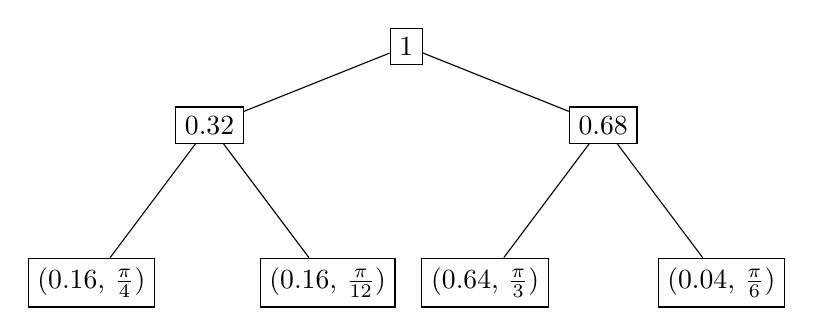
\begin{tikzpicture}[
  every node/.style={rectangle, draw},
  level 1/.style={sibling distance=50mm, level distance=10mm},
  level 2/.style={sibling distance=30mm, level distance=20mm}
]
\node {1}
  child {node {0.32}
    child {node {(0.16, $\frac{\pi}{4}$)}}
    child {node {(0.16, $\frac{\pi}{12}$)}}
  }
  child {node {0.68}
    child {node {(0.64, $\frac{\pi}{3}$)}}
    child {node {(0.04, $\frac{\pi}{6}$)}}
  }; 
\end{tikzpicture}
\hspace{1cm} % Adjust horizontal space between trees here
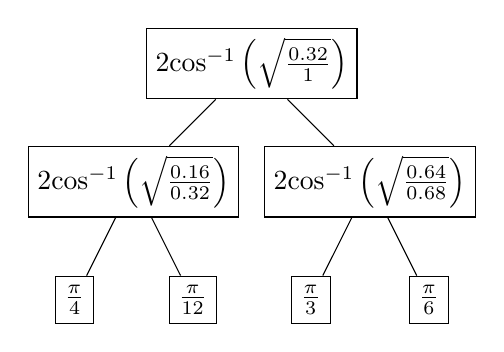
\begin{tikzpicture}[
  every node/.style={rectangle, draw},
  level 1/.style={sibling distance=30mm, level distance=15mm},
  level 2/.style={sibling distance=15mm, level distance=15mm}
]
\node {$2\text{cos}^{-1}\left(\sqrt{\frac{0.32}{1}} \right)$}
  child {node {$2\text{cos}^{-1}\left(\sqrt{\frac{0.16}{0.32}} \right)$}
    child {node {$\frac{\pi}{4}$}}
    child {node {$\frac{\pi}{12}$}}
  }
  child {node {$2\text{cos}^{-1}\left(\sqrt{\frac{0.64}{0.68}} \right)$}
    child {node {$\frac{\pi}{3}$}}
    child {node {$\frac{\pi}{6}$}}
  }; 
\end{tikzpicture}

\begin{tikzpicture}[overlay, remember picture]
  \draw[->,thick] (8,2.5) -- (10,2.5);
\end{tikzpicture}
\end{figure}

\end{document}
